% Options for packages loaded elsewhere
\PassOptionsToPackage{unicode}{hyperref}
\PassOptionsToPackage{hyphens}{url}
%
\documentclass[
]{book}
\usepackage{lmodern}
\usepackage{amssymb,amsmath}
\usepackage{ifxetex,ifluatex}
\ifnum 0\ifxetex 1\fi\ifluatex 1\fi=0 % if pdftex
  \usepackage[T1]{fontenc}
  \usepackage[utf8]{inputenc}
  \usepackage{textcomp} % provide euro and other symbols
\else % if luatex or xetex
  \usepackage{unicode-math}
  \defaultfontfeatures{Scale=MatchLowercase}
  \defaultfontfeatures[\rmfamily]{Ligatures=TeX,Scale=1}
\fi
% Use upquote if available, for straight quotes in verbatim environments
\IfFileExists{upquote.sty}{\usepackage{upquote}}{}
\IfFileExists{microtype.sty}{% use microtype if available
  \usepackage[]{microtype}
  \UseMicrotypeSet[protrusion]{basicmath} % disable protrusion for tt fonts
}{}
\makeatletter
\@ifundefined{KOMAClassName}{% if non-KOMA class
  \IfFileExists{parskip.sty}{%
    \usepackage{parskip}
  }{% else
    \setlength{\parindent}{0pt}
    \setlength{\parskip}{6pt plus 2pt minus 1pt}}
}{% if KOMA class
  \KOMAoptions{parskip=half}}
\makeatother
\usepackage{xcolor}
\IfFileExists{xurl.sty}{\usepackage{xurl}}{} % add URL line breaks if available
\IfFileExists{bookmark.sty}{\usepackage{bookmark}}{\usepackage{hyperref}}
\hypersetup{
  pdftitle={Analyse multidimensionnelle appliquée},
  pdfauthor={Denis Larocque, Léo Belzile},
  hidelinks,
  pdfcreator={LaTeX via pandoc}}
\urlstyle{same} % disable monospaced font for URLs
\usepackage{longtable,booktabs}
% Correct order of tables after \paragraph or \subparagraph
\usepackage{etoolbox}
\makeatletter
\patchcmd\longtable{\par}{\if@noskipsec\mbox{}\fi\par}{}{}
\makeatother
% Allow footnotes in longtable head/foot
\IfFileExists{footnotehyper.sty}{\usepackage{footnotehyper}}{\usepackage{footnote}}
\makesavenoteenv{longtable}
\usepackage{graphicx,grffile}
\makeatletter
\def\maxwidth{\ifdim\Gin@nat@width>\linewidth\linewidth\else\Gin@nat@width\fi}
\def\maxheight{\ifdim\Gin@nat@height>\textheight\textheight\else\Gin@nat@height\fi}
\makeatother
% Scale images if necessary, so that they will not overflow the page
% margins by default, and it is still possible to overwrite the defaults
% using explicit options in \includegraphics[width, height, ...]{}
\setkeys{Gin}{width=\maxwidth,height=\maxheight,keepaspectratio}
% Set default figure placement to htbp
\makeatletter
\def\fps@figure{htbp}
\makeatother
\setlength{\emergencystretch}{3em} % prevent overfull lines
\providecommand{\tightlist}{%
  \setlength{\itemsep}{0pt}\setlength{\parskip}{0pt}}
\setcounter{secnumdepth}{5}
% \usepackage[mathscr]{eucal}
\DeclareMathAlphabet{\mathcrl}{U}{rsfs}{m}{n}

% \DeclareMathAlphabet{\mathcal}{OMS}{cmsy}{m}{n}
\usepackage{booktabs}
\usepackage[left=1.2in, right= 1.2in]{geometry}
\makeatletter
\def\thm@space@setup{%
  \thm@preskip=8pt plus 2pt minus 4pt
  \thm@postskip=\thm@preskip
}
\makeatother

% \AtBeginDocument{

% \geometry{left=1.2in, right= 1.2in}
\usepackage{fourier}
\usepackage[french]{babel}
% }
\usepackage[]{natbib}
\bibliographystyle{apalike}

\title{Analyse multidimensionnelle appliquée}
\author{Denis Larocque, Léo Belzile}
\date{Version du 2020-01-24}

\usepackage{amsthm}
\newtheorem{theorem}{Théorème}[chapter]
\newtheorem{lemma}{Lemme}[chapter]
\newtheorem{corollary}{Corollaire}[chapter]
\newtheorem{proposition}{Proposition}[chapter]
\newtheorem{conjecture}{Conjecture}[chapter]
\theoremstyle{definition}
\newtheorem{definition}{Définition}[chapter]
\theoremstyle{definition}
\newtheorem{example}{Exemple}[chapter]
\theoremstyle{definition}
\newtheorem{exercise}{Exercice}[chapter]
\theoremstyle{remark}
\newtheorem*{remark}{Remarque}
\newtheorem*{solution}{Solution}
\let\BeginKnitrBlock\begin \let\EndKnitrBlock\end
\begin{document}
\frontmatter
\maketitle

{
\setcounter{tocdepth}{1}
\tableofcontents
}
\mainmatter
\newcommand{\bs}[1]{\boldsymbol{#1}}
\newcommand{\eps}{\varepsilon}
\newcommand{\Rlang}{\textsf{R}}
\newcommand{\SAS}{\textsf{SAS}}
\newcommand{\Sp}{\mathscr{S}}
\newcommand{\E}[1]{{\mathsf E}\left(#1\right)}
\newcommand{\Va}[1]{{\mathsf{Var}}\left(#1\right)}
\newcommand{\Cor}[1]{{\mathsf{Cor}}\left(#1\right)}
\newcommand{\I}[1]{{\mathbf 1}_{#1}}

\hypertarget{introduction}{%
\chapter{Introduction}\label{introduction}}

\hypertarget{survol-du-cours}{%
\section{Survol du cours}\label{survol-du-cours}}

\hypertarget{analyse-factorielle-exploratoire}{%
\subsection{Analyse factorielle exploratoire}\label{analyse-factorielle-exploratoire}}

On dispose de \(p\) variables \(X_1, \ldots, X_p\). Peut-on expliquer les interrelations (la structure de corrélation) entre ces variables à l'aide d'un certain nombre (moins de \(p\)) de facteurs latents (non observés)?

L'analyse factorielle est souvent utilisée pour analyser des questionnaires (construction d'échelles) comme dans l'exemple suivant.

\BeginKnitrBlock{example}
\protect\hypertarget{exm:unnamed-chunk-1}{}{\label{exm:unnamed-chunk-1} }Pour les besoins d'une enquête, on a demandé à 200 consommateurs adultes de répondre aux questions suivantes par rapport à un certain type de magasin:

Sur une échelle de 1 à 5,

\begin{enumerate}
\def\labelenumi{\arabic{enumi}.}
\tightlist
\item
  pas important
\item
  peu important
\item
  moyennement important
\item
  assez important
\item
  très important
\end{enumerate}

Pour vous, à quel point est-ce important\ldots

\begin{enumerate}
\def\labelenumi{\arabic{enumi}.}
\tightlist
\item
  que le magasin offre de bons prix tous les jours?
\item
  que le magasin accepte les cartes de crédit majeures (Visa, Mastercard)?
\item
  que le magasin offre des produits de qualité?
\item
  que les vendeurs connaissent bien les produits?
\item
  qu'il y ait des ventes spéciales régulièrement?
\item
  que les marques connues soient disponibles?
\item
  que le magasin ait sa propre carte de crédit?
\item
  que le service soit rapide?
\item
  qu'il y ait une vaste sélection de produits?
\item
  que le magasin accepte le paiement par carte de débit?
\item
  que le personnel soit courtois?
\item
  que le magasin ait en stock les produits annoncés?
\end{enumerate}

Pouvons-nous identifier un nombre restreint de facteurs (concepts, dimensions) qui pourraient bien rendre compte de la structure de corrélation entre ces 12 variables?
\EndKnitrBlock{example}

Buts:

\begin{itemize}
\tightlist
\item
  Décrire et comprendre la structure de corrélation d'un ensemble de variables à l'aide d'un nombre restreint de concepts (appelés facteurs).
\item
  Réduire le nombre de variables en créant une nouvelle variable par facteur. Ces nouvelles variables pourront par la suite être utilisées dans d'autres analyses (régression linéaire multiple par exemple).
\end{itemize}

\hypertarget{suxe9lection-de-variables-et-de-moduxe8les}{%
\subsection{Sélection de variables et de modèles}\label{suxe9lection-de-variables-et-de-moduxe8les}}

Dans plusieurs situations, on doit développer un modèle de prévision. Par exemple, on pourrait devoir développer un modèle pour:

\begin{itemize}
\tightlist
\item
  Détecter les faillites des clients (ou des entreprises)
\item
  Cibler les clients qui seront intéressés par une offre promotionnelle
\item
  Détecter les fraudes (par carte de crédit ou dans les rapports de revenus)
\item
  Prévoir si un client va nous quitter.
\end{itemize}

Il y a en général plusieurs variables explicatives potentielles, et aussi plusieurs types de modèles possibles (régression linéaire, réseaux de neurones, arbres de régression ou de classification, etc.). Dans ce chapitre, nous verrons des principes généraux et des outils afin de sélectionner des modèles performants, ou bien un sous-ensemble de variables avec un bon pouvoir prévisionnel.

\hypertarget{ruxe9gression-logistique}{%
\subsection{Régression logistique}\label{ruxe9gression-logistique}}

On cherche à expliquer le comportement d'une variable binaire \(Y\) (\(0-1\)), à l'aide de \(p\) variables quelconques \(X_1, \ldots, X_p\).

\BeginKnitrBlock{example}
\protect\hypertarget{exm:unnamed-chunk-2}{}{\label{exm:unnamed-chunk-2} }Une banque offre aux gens la possibilité de faire une demande de carte de crédit en ligne en promettant une approbation (conditionnelle) en quelques minutes seulement. Le tout est basé sur un modèle automatique de classification qui décide d'accorder ou non la carte (\(Y=1\) ou \(Y=0\)) en fonction des réponses fournies par les clients potentiels à différentes questions comme: quel est votre revenu annuel brut (\(X_1\)), avez-vous d'autres cartes de crédit (\(X_2\)), êtes-vous locataire ou propriétaire (\(X_3\)), etc\ldots
\EndKnitrBlock{example}

Buts:

\begin{itemize}
\tightlist
\item
  Comprendre comment et dans quelle mesure les variables \(\boldsymbol{X}\) influencent la catégorie d'appartenance de \(Y\).
\item
  Développer un modèle pour faire de la classification, c'est-à-dire, prévoir la catégorie d'appartenance de \(Y\) pour un nouveau sujet à partir des variables \(\boldsymbol{X}\).
\end{itemize}

\hypertarget{analyse-de-regroupements}{%
\subsection{Analyse de regroupements}\label{analyse-de-regroupements}}

On cherche à créer des groupes (« \emph{clusters} ») d'individus homogènes en utilisant \(p\) variables \(X_1, \ldots, X_p\).

\BeginKnitrBlock{example}
\protect\hypertarget{exm:unnamed-chunk-3}{}{\label{exm:unnamed-chunk-3} }
Cette méthode est utilisée en marketing pour la \textbf{segmentation de marché}, qui consiste en

\begin{quote}
\ldots définir des sous-groupes réunissant des consommateurs qui partagent les mêmes préférences ou qui réagissent de façon semblable à des variables de marketing\footnote{d'Astous, A. (2000). \emph{Le projet de recherche en marketing}, 2e édition. Chenelière/McGraw-Hill. }
\end{quote}
\EndKnitrBlock{example}

But:

\begin{itemize}
\tightlist
\item
  Combiner des sujets en groupes (interprétables) de telle sorte que les individus d'un même groupe soient les plus semblables possible par rapport à certaines caractéristiques et que les groupes soient les plus différents possible.
\end{itemize}

\hypertarget{analyse-de-survie}{%
\subsection{Analyse de survie}\label{analyse-de-survie}}

On s'intéresse au temps avant qu'un événement survienne. Par exemple :

\begin{itemize}
\tightlist
\item
  Temps qu'un client demeure abonné à un service offert par notre compagnie.
\item
  Temps de survie d'un individu après avoir été diagnostiqué avec un certain type de cancer.
\item
  Temps qu'un employé demeure au service de la compagnie.
\item
  Temps qu'une franchise demeure en activité.
\item
  Temps avant la faillite d'une entreprise (ou d'un particulier).
\item
  Temps avant le prochain achat d'un client.
\end{itemize}

On observe chaque sujet jusqu'à ce que l'une des deux choses suivantes se produise: l'événement survient avant la fin de la période d'observation ou bien l'étude se termine et l'événement n'est toujours pas survenu. Dans le premier exemple, l'événement correspond au fait d'interrompre son abonnement. On dispose donc d'une variable temps \(T\) pour chaque individu qui est soit censurée, soit non censurée. Si l'individu a expérimenté l'événement avant la fin de la période d'observation, la valeur de est non censurée. Si l'événement n'est toujours pas survenu à la fin de la période d'observation, la valeur de \(T\) est censurée. Pour chaque individu, on dispose également d'un ensemble de variables explicatives \(X_1, \ldots, X_p\).

But:

\begin{itemize}
\tightlist
\item
  Étudier les effets des variables explicatives sur le temps de survie et obtenir des prévisions du temps de survie.
\end{itemize}

\hypertarget{donnuxe9es-manquantes}{%
\subsection{Données manquantes}\label{donnuxe9es-manquantes}}

Il arrive fréquemment d'avoir des valeurs manquantes dans notre échantillon.

Simplement ignorer les sujets avec des valeurs manquantes et faire l'analyse avec les autres sujets conduit généralement à des estimations biaisées et à de l'inférence invalide.

Dans ce chapitre, nous verrons une méthode très générale afin de traiter les données manquantes, l'imputation multiple. Nous verrons comment elle peut être utilisée dans un contexte d'inférence et dans un contexte de prévision.

\hypertarget{analyse-factorielle-exploratoire-1}{%
\chapter{Analyse factorielle exploratoire}\label{analyse-factorielle-exploratoire-1}}

\hypertarget{introduction-1}{%
\section{Introduction}\label{introduction-1}}

On dispose de \(p\) variables \(X_1, \ldots, X_p\).

\begin{itemize}
\tightlist
\item
  Y a-t-il des groupements de variables?
\item
  Est-ce que les variables faisant partie d'un groupement semblent mesurer certains aspects d'un facteur commun (non observé)?
\end{itemize}

Un tel groupement peut être détecté si plusieurs variables sont très corrélées entre elles. Est-ce que la structure de corrélation entre les \(p\) variables peut être expliquée à l'aide d'un nombre restreint de facteurs?

\emph{Exemple de facteurs}: Habileté quantitative, habileté sociale, importance accordée à la qualité du service, importance accordée à la loyauté, habileté de leader, etc\ldots

L'analyse factorielle est aussi une méthode de réduction du nombre de variables. En effet, une fois qu'on a identifié les facteurs, on peut remplacer les variables individuelles par un résumé pour chaque facteur (qui est souvent la moyenne des variables qui font partie du facteur).

Pour faire une analyse factorielle, la taille d'échantillon devrait être d'au moins 10 fois le nombre de variables.

\hypertarget{rappels-sur-le-coefficient-de-corruxe9lation-linuxe9aire}{%
\section{Rappels sur le coefficient de corrélation linéaire}\label{rappels-sur-le-coefficient-de-corruxe9lation-linuxe9aire}}

On veut examiner la relation entre deux variables \(X\) et \(Y\) et on dispose de \(n\) couples d'observations, où \(x_i\) (\(y_i\)) est la valeur de la variable \(X\) (\(Y\)) pour le \(i\)e individu.

Le coefficient de corrélation linéaire, que l'on note \(r\), cherche à mesurer la force de la relation linéaire entre deux variables, c'est-à-dire à quantifier à quel point les observations sont alignées autour d'une droite. Le coefficient de corrélation est
\begin{align*}
r = \frac{\sum_{i=1}^n (x_i-\overline{x})(y_i -\bar{y})}{\left\{\sum_{i=1}^n (x_i-\overline{x})^2 \sum_{i=1}^n(y_i -\bar{y})^2\right\}^{1/2}}
\end{align*}

Les propriétés les plus importantes du coefficient de corrélation linéaire sont les suivantes:

\begin{enumerate}
\def\labelenumi{\arabic{enumi})}
\tightlist
\item
  \(-1 \leq r \leq 1\);
\item
  \(r=1\) (respectivement \(r=-1\)) si et seulement si les \(n\) observations sont exactement alignées sur une droite de pente positive (négative). C'est-à-dire, s'il existe deux constantes \(a\) et \(b>0\) (\(b<0\)) telles que \(y_i=a+b x_i\) pour tout \(i=1, \ldots, n\).
\end{enumerate}

Règle générale,

\begin{itemize}
\tightlist
\item
  Plus la corrélation est près de 1, plus les points auront tendance à être alignés autour d'une droite de pente positive. Par conséquent, plus la valeur de \(X\) augmente, plus celle de \(Y\) aura tendance à augmenter et vice-versa.
\item
  Plus la corrélation est près de \(-1\), plus les points auront tendance à être alignés autour d'une droite de pente négative. Par conséquent, plus la valeur de \(X\) augmente, plus celle de \(Y\) aura tendance à diminuer et vice-versa.
\item
  Lorsque la corrélation est presque nulle, les points n'auront pas tendance à être alignés autour d'une droite. Il est très important de noter que cela n'implique pas qu'il n'y a pas de relation entre les deux variables. Cela implique seulement qu'il n'y a pas de \textbf{relation linéaire} entre les deux variables.
\end{itemize}

\hypertarget{exemple-de-questionnaire}{%
\section{Exemple de questionnaire}\label{exemple-de-questionnaire}}

Le questionnaire suivant porte sur une étude dans un magasin. Pour les besoins d'une enquête, on a demandé à 200 consommateurs adultes de répondre aux questions suivantes par rapport à un certain type de magasin sur une échelle de 1 à 5, où

\begin{enumerate}
\def\labelenumi{\arabic{enumi}.}
\tightlist
\item
  pas important
\item
  peu important
\item
  moyennement important
\item
  assez important
\item
  très important
\end{enumerate}

Pour vous, à quel point est-ce important\ldots

\begin{enumerate}
\def\labelenumi{\arabic{enumi}.}
\tightlist
\item
  que le magasin offre de bons prix tous les jours?
\item
  que le magasin accepte les cartes de crédit majeures (Visa, Mastercard)?
\item
  que le magasin offre des produits de qualité?
\item
  que les vendeurs connaissent bien les produits?
\item
  qu'il y ait des ventes spéciales régulièrement?
\item
  que les marques connues soient disponibles?
\item
  que le magasin ait sa propre carte de crédit?
\item
  que le service soit rapide?
\item
  qu'il y ait une vaste sélection de produits?
\item
  que le magasin accepte le paiement par carte de débit?
\item
  que le personnel soit courtois?
\item
  que le magasin ait en stock les produits annoncés?
\end{enumerate}

Une analyse factorielle cherchera à identifier automatiquement des groupes de variables qui sont fortement corrélées entre elles.

Les commandes \textsf{SAS}(ainsi que plusieurs commentaires) pour faire les analyses se trouvent dans le fichier \texttt{factor1\_intro.sas}. Les statistiques descriptives ainsi que la matrice des corrélations sont obtenues en exécutant les lignes suivantes:

\begin{verbatim}
proc corr data=multi.factor2;
var x1-x12;
run;
\end{verbatim}

\begin{center}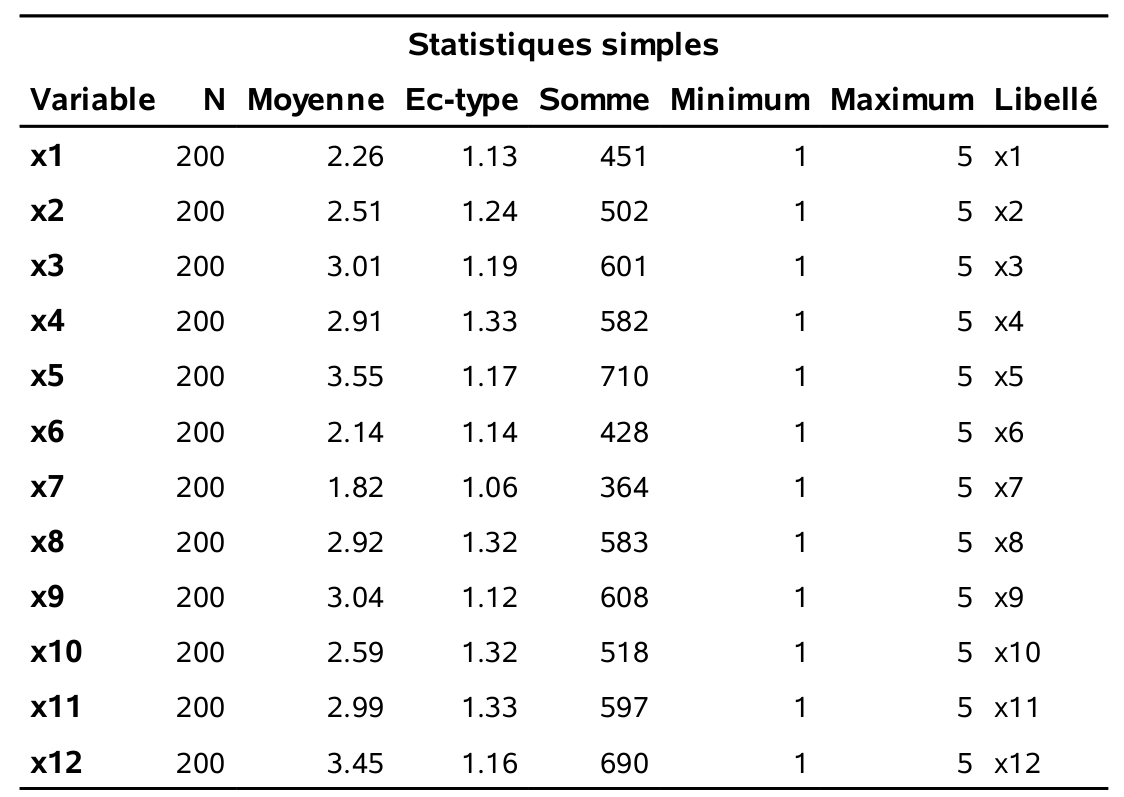
\includegraphics[width=0.9\linewidth]{figures/01-facto-e1} \end{center}

\begin{center}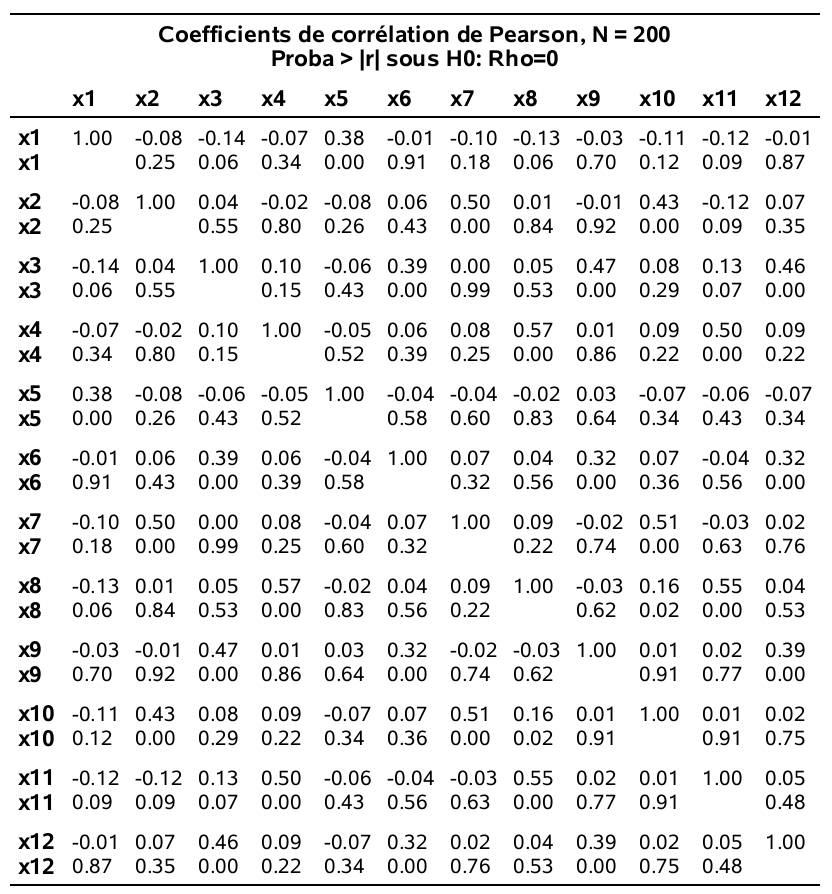
\includegraphics[width=0.9\linewidth]{figures/01-facto-e2} \end{center}

\hypertarget{description-du-moduxe8le-danalyse-factorielle}{%
\section{Description du modèle d'analyse factorielle}\label{description-du-moduxe8le-danalyse-factorielle}}

On dispose d'observations sur \(p\) variables \(X_1, \ldots, X_p\). Le modèle d'analyse factorielle fait l'hypothèse que ces variables dépendent linéairement d'un plus petit nombre \(m\) de variables aléatoires, \(F_1, \ldots, F_m\), appelées facteurs communs et de \(p\) termes d'erreurs (ou facteurs spécifiques) \(\varepsilon_1, \ldots, \varepsilon_p\), de moyenne \({\mathsf E}\left(\varepsilon_i\right)=0\) et de variance \({\mathsf{Var}}\left(\varepsilon_i\right)=\psi_i\) pour \(i=1, \ldots, p\). Spécifiquement, le modèle est
\begin{align*}
X_1 &= \mu_1 + l_{11}F_1 + l_{12} F_2 + \cdots + l_{1m}F_m + \varepsilon_1\\
X_2 &= \mu_2 + l_{21}F_1 + l_{22} F_2 + \cdots + l_{2m}F_m + \varepsilon_2\\
&\vdots \\
X_p &= \mu_p + l_{p1}F_1 + l_{p2} F_2 + \cdots + l_{pm}F_m + \varepsilon_p,
\end{align*}
où \(\mu_i\) est l'espérance de la variable aléatoire \(X_i\) (\(i=1, \ldots, p\)) et où \(l_{ij}\) est le chargement de la variable \(X_i\) sur le facteur \(F_j\) (\(i=1,\ldots, p; j=1, \ldots, m\)).

Les espérances (\(\mu_i\)), les chargements (\(l_{ij}\)) et les variances (\(\psi_i\)) sont des quantités fixes, mais inconnues, tandis que les facteurs communs (\(F_i\)) et spécifiques (\(\varepsilon_i\)) sont des variables aléatoires non observables.

Des hypothèses supplémentaires sont nécessaires afin de pouvoir utiliser ce modèle (contraintes d'identifiabilité des paramètres). Sans entrer dans les détails, mentionnons que l'une de ces hypothèses est que les facteurs sont non corrélés.

De plus, si les variables ont été préalablement standardisées de telle sorte que \({\mathsf E}\left(X_i\right)=0\) et \({\mathsf{Var}}\left(X_i\right)=1\) (note: ceci revient à utiliser la matrice de corrélation des observations dans l'analyse ce qui est fait par défaut dans \textsf{SAS}), alors \({\mathsf{Cor}}\left(X_i, F_j\right)=l_{ij}\), c'est-à-dire, le chargement de la variable \(X_i\) sur le chargement \(F_j\) est le coefficient de corrélation entre cette variable et ce facteur.

Sans aucune contrainte sur le modèle, la matrice de covariance de \(X_1, \ldots, X_p\) possède \(p(p+1)/2\) paramètres, soit \(p\) variances et \(p(p-1)/2\) termes de corrélation. Avec le modèle d'analyse factorielle, on suppose que l'on peut décrire cette structure en utilisant seulement \(p(m+1)\) paramètres (\(p\) variances spécifiques et \(pm\) chargements). Par exemple, avec \(p=50\) variables et \(m=6\) facteurs, on essaie de décrire la structure de covariance à l'aide de 350 paramètres au lieu de 1275.

Il existe plusieurs méthodes pour extraire les facteurs, c'est-à-dire pour estimer les paramètres du modèle (les \(\psi_i\) et les \(l_{ij}\)). Nous allons discuter de deux d'entre elles: la méthode du maximum de vraisemblance et la méthode des composantes principales. L'avantage de l'estimation par maximum de vraisemblance est qu'elle permet l'utilisation de critères d'information et de statistiques de tests pour guider le choix du nombre de facteurs. En revanche, l'estimation des paramètres requiert une optimisation numérique qui peut être délicate selon les cas de figure.

\hypertarget{rotation-des-facteurs}{%
\subsection{Rotation des facteurs}\label{rotation-des-facteurs}}

Dans le modèle d'analyse factorielle, on peut montrer que, lorsqu'il y a deux facteurs ou plus, il existe plusieurs configurations de facteurs qui donnent la même structure de covariance. En fait, les chargements peuvent seulement être déterminés à une transformation orthogonale prêt (note: une transformation orthogonale est une transformation qui préserve le produit scalaire; elle préserve ainsi toutes les distances et les angles entre deux vecteurs). Si les chargements provenant d'une méthode d'extraction des facteurs ne sont pas uniques, la matrice de corrélation estimée par le modèle est par contre unique.

Il existe plusieurs techniques de rotation de facteurs. Le but de ces techniques est d'essayer de trouver une solution qui fera en sorte que les facteurs seront facilement interprétables. La méthode la plus utilisée est la méthode \textbf{varimax}: elle produit une configuration de chargement en maximisant la variance de la somme des carrés des chargements pour les \(m\) facteurs. La méthode varimax tend à produire une configuration de facteurs tel que les chargements de chaque variable sont dispersés (des chargements élevés positifs ou négatifs et d'autres presque nuls).

Je vous suggère de toujours tenter d'interpréter la solution avec une rotation varimax. Si ce n'est pas suffisamment clair, il existe d'autres méthodes de rotation dont certaines (les rotations de type oblique) permettent la présence de corrélation entre les facteurs.

\hypertarget{estimation-des-facteurs}{%
\section{Estimation des facteurs}\label{estimation-des-facteurs}}

Les chargements estimés pour la solution à quatre facteurs, suite à la rotation varimax, sont obtenus avec le code SAS suivant:

\begin{verbatim}
proc factor data=multi.factor2 
 method=ml rotate=varimax nfact=4
 maxiter=500 flag=.3 hey;
 var x1-x12;
run;
\end{verbatim}

\begin{center}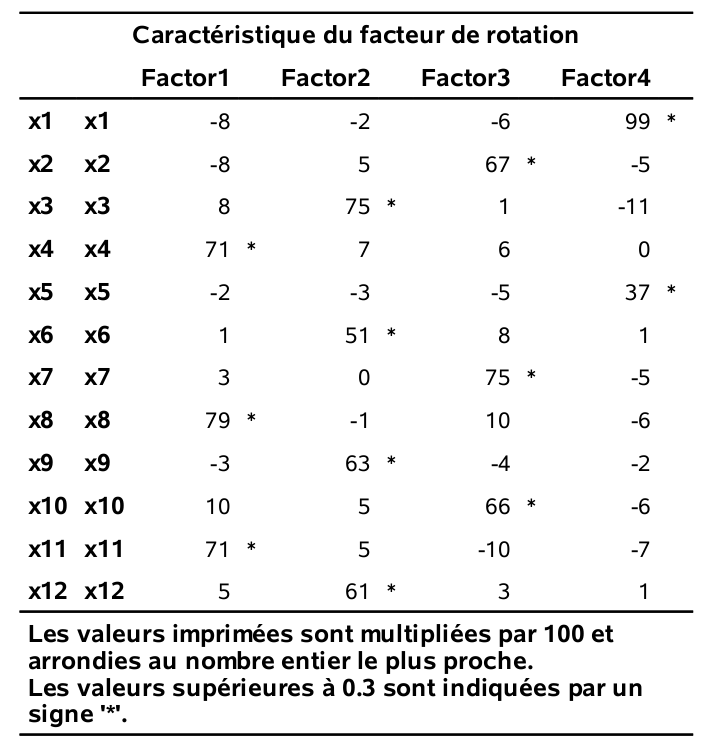
\includegraphics[width=0.7\linewidth]{figures/01-facto-e3} \end{center}

En général, on associe une variable à un groupe (facteur) si son chargement est supérieur à 0,3 (en valeur absolue), ce qui donne

\begin{itemize}
\tightlist
\item
  Facteur 1: \(X_4\),\(X_8\) et \(X_{11}\)
\item
  Facteur 2: \(X_3\),\(X_6\), \(X_9\) et \(X_{12}\)
\item
  Facteur 3: \(X_2\),\(X_7\) et \(X_{10}\)
\item
  Facteur 4: \(X_1\) et \(X_5\).
\end{itemize}

Ces facteurs sont interprétables:

\begin{itemize}
\tightlist
\item
  Le facteur 1 représente l'importance accordée au service.
\item
  Le facteur 2 représente l'importance accordée aux produits.
\item
  Le facteur 3 représente l'importance accordée à la facilité de paiement.
\item
  Le facteur 4 représente l'importance accordée aux prix.
\end{itemize}

Dans cet exemple, les choses se sont bien passées et le nombre de facteurs que nous avons spécifié (4) semble être adéquat, mais ce n'est pas toujours aussi évident. Il est utile d'avoir des outils pour guider le choix du nombre de facteurs.

\hypertarget{choix-du-nombre-de-facteurs}{%
\section{Choix du nombre de facteurs}\label{choix-du-nombre-de-facteurs}}

Il existe différentes méthodes pour se guider dans le nombre de facteurs, \(m\), à utiliser. Cependant, le point important à retenir est que, peu importe le nombre choisi, il faut que les facteurs soient \textbf{interprétables}. Par conséquent, les méthodes qui
suivent ne devraient servir que de guide et non pas être suivies aveuglément.
La méthode du maximum de vraisemblance que nous avons utilisée dans l'exemple possède l'avantage de fournir trois critères pour choisir le nombre de facteurs appropriés. Ces critères sont:

\begin{itemize}
\tightlist
\item
  AIC (critère d'information d'Akaike)
\item
  BIC (critère d'information bayésien de Schwarz)
\item
  Le test du rapport de vraisemblance pour l'hypothèse nulle que le modèle de corrélation décrit le modèle factoriel avec \(m\) facteurs est adéquat, contre l'alternative qu'il n'est pas adéquat.
\end{itemize}

Les critères d'information servent à la sélection de modèles; ils seront traités plus en détail dans les chapitres qui suivent. Pour l'instant, il est suffisant de savoir que le modèle avec la valeur du critère AIC (ou BIC) la plus petite est considéré le « meilleur » (selon ce critère).

Les sorties suivantes proviennent du même programme SAS et correspondent au modèle factoriel avec quatre facteurs estimé par maximum de vraisemblance.

\begin{center}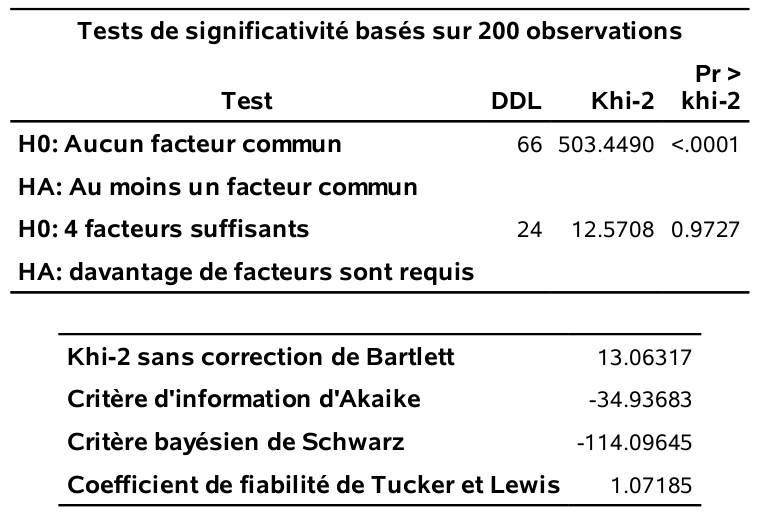
\includegraphics[width=0.7\linewidth]{figures/01-facto-e4} \end{center}

Pour choisir le nombre de facteurs avec les critères, il faut ajuster le modèle en faisant varier le nombre de facteurs (option \texttt{nfact} et extraire la valeur numérique.

Le tableau @ref(01-IC\_table) présente les valeurs estimées des critères d'information et des valeurs-\(p\) pour le test du rapport de vraisemblance pour cinq modèles. Le critère AIC suggère quatre facteurs, tandis que les deux autres critères (BIC et test du rapport de vraisemblance suggèrent plutôt trois facteurs.

\begin{longtable}[]{@{}crrr@{}}
\toprule
m & AIC & BIC & valeur-\emph{p}\tabularnewline
\midrule
\endhead
1 & 228,0 & 49,9 & \textless0,001\tabularnewline
2 & 99,5 & -42,3 & \textless0,001\tabularnewline
3 & -20,5 & -129,3 & 0,096\tabularnewline
4 & -34,9 & -114,1 & 0,973\tabularnewline
5 & -24,8 & -77,6 & 0,975\tabularnewline
\bottomrule
\end{longtable}

On peut considérer le modèle avec trois facteurs: les chargements (après rotation varimax) sont données dans le tableau \ref{fig:fig1p5}.

\begin{figure}

{\centering 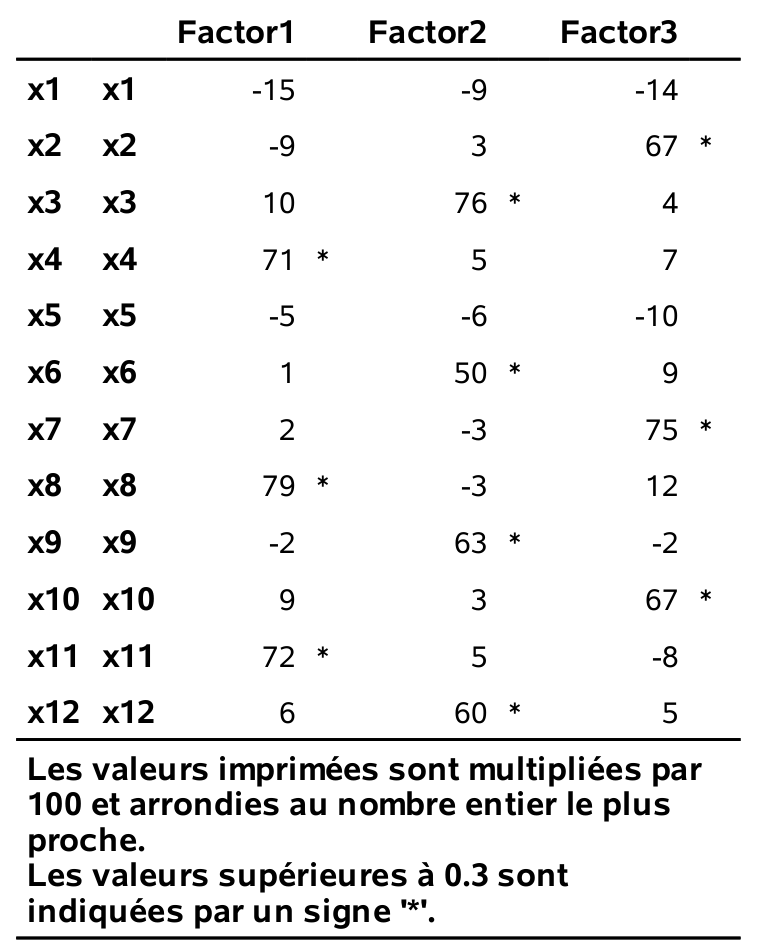
\includegraphics[width=0.55\linewidth]{figures/01-facto-e5} 

}

\caption{Estimés des chargements pour trois facteurs avec rotation varimax}\label{fig:fig1p5}
\end{figure}

Cette solution récupère les trois facteurs \emph{service}, \emph{produits} et \emph{paiement} de la solution précédente à quatre facteurs. Le facteur \emph{prix} (qui était formé de \(X_1\) et \(X_5\)) n'est plus présent: que faire avec ce dernier? Cela dépend du but de l'analyse et nous y reviendrons plus tard.

Pour terminer cette section, voici la description de deux autres
critères \emph{classiques} pour choisir le nombre de facteurs. Ces deux critères sont:

\begin{itemize}
\tightlist
\item
  Critère de Kaiser, un critère basé sur les valeurs propres. Avec une analyse en composantes principales basée sur la matrice des corrélations, la valeur propre associée à un facteur représente la partie de la variance totale qui est expliquée par ce facteur. Chaque variable compte pour un dans la variance totale. Le nombre de facteurs choisis est le nombre de valeurs propres supérieures à 1. L'idée est de garder seulement les facteurs qui expliquent plus de variance qu'une variable individuelle.
\item
  le diagramme d'éboulis: un graphique des valeurs propres ordonnées de la plus grande à la plus petite en fonction de \(1,\ldots, p\). Habituellement, ce graphe prendra la forme d'une chute assez importante suivie d'une stabilisation des valeurs propres. Avec ce critère, le nombre de facteurs est déterminé par le nombre de valeurs propres avant le début du coude où il a stabilisation apparente. L'idée est de choisir l'endroit où l'ajout d'un facteur supplémentaire n'apporte qu'un gain marginal faible. Ce critère est par contre subjectif et dépend de l'analyste.
\end{itemize}

Les sorties qui suivent proviennent du programme:

\begin{verbatim}
proc factor data=multi.factor2 method=principal
 scree rotate=varimax flag=.3;
var x1-x12;
run;
\end{verbatim}

Cette fois-ci, c'est la méthode des composantes principales qui
est utilisée (voir section suivante). En ne spécifiant pas l'option \texttt{nfact}, \textsf{SAS}choisit le nombre de facteurs en utilisant par défaut le critère de Kaiser (valeurs propres supérieures à 1). Quatre facteurs sont retenus, tel qu'indiqué par la sortie au bas du tableau \ref{fig:fig1p7}. Pour le diagramme d'éboulis de la figure \ref{fig:fig1p6}, le choix est assez subjectif: il semble raisonnable de choisir trois ou quatre facteurs.

\begin{figure}

{\centering 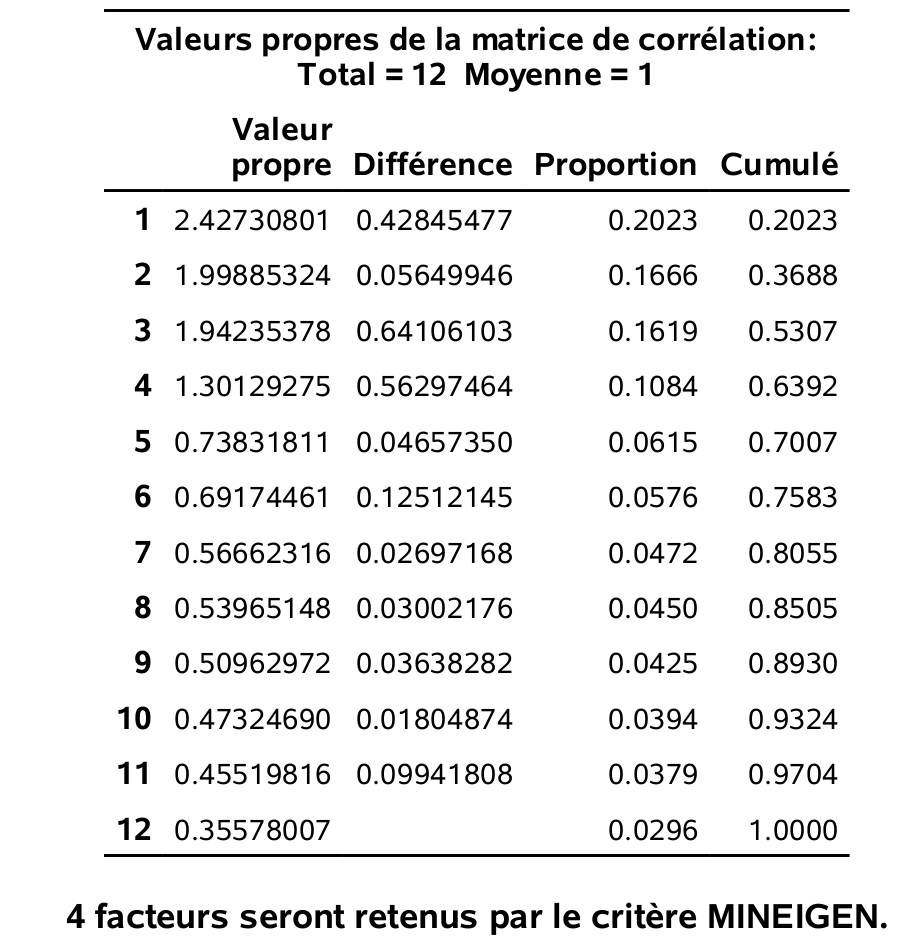
\includegraphics[width=0.65\linewidth]{figures/01-facto-e7} 

}

\caption{Valeurs propres et proportion de variance}\label{fig:fig1p7}
\end{figure}

\begin{figure}

{\centering 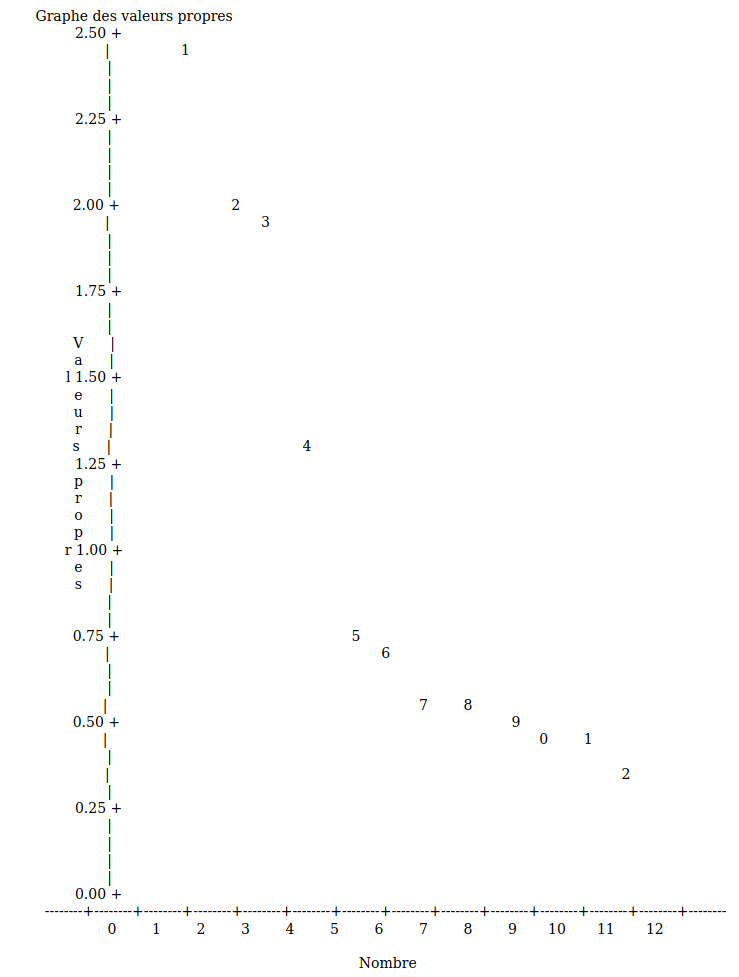
\includegraphics[width=0.65\linewidth]{figures/01-facto-e6} 

}

\caption{Diagramme d'éboulis}\label{fig:fig1p6}
\end{figure}

On suggère d'utiliser \emph{de facto} les trois critères découlant de l'utilisation de la vraisemblance et de déterminer le nombre de facteurs à extraire selon différents critères avant d'examiner les modèles avec ce nombre de facteurs et ceux
avec un facteur de moins ou de plus. Au final, le plus important est de pouvoir interpréter raisonnablement les facteurs et donc le modèle retenu est souvent choisi selon le critère \textbf{Wow!}. On veut dire par là que la configuration de facteurs choisie est compréhensible.

\hypertarget{construction-duxe9chelles-uxe0-partir-des-facteurs}{%
\section{Construction d'échelles à partir des facteurs}\label{construction-duxe9chelles-uxe0-partir-des-facteurs}}

Si le seul but de l'analyse factorielle est de comprendre la structure de corrélation entre les variables, alors se limiter à l'interprétation des facteurs est suffisant.

Si par contre, le but est de réduire le nombre de variables pour pouvoir par la suite procéder à d'autres analyses statistiques, l'analyse factorielle peut alors servir de guide pour construire de nouvelles variables (échelles). En supposant que l'analyse factorielle a produit des facteurs qui sont interprétables et satisfaisants, la méthode de construction d'échelles la plus couramment utilisée consiste à construire \(m\) nouvelles variables, une par facteur. Pour un facteur donné, la nouvelle variable est simplement la moyenne des variables ayant des chargements élevés sur ce facteur (positifs ou négatifs, mais de même signe). Une autre méthode, les scores factoriels, sera présentée plus loin.

Lorsqu'on construit une échelle, il est important d'examiner sa cohérence interne. Ceci peut être fait à l'aide du coefficient alpha de Cronbach. Ce coefficient mesure à quel point chaque variable faisant partie d'une échelle est corrélée avec le total de toutes les variables pour cette échelle.
Plus le coefficient est élevé, plus les variables ont tendance à être corrélées entre elles. L'alpha de Cronbach est
\begin{align*}
\alpha=\frac{k}{k-1} \frac{S^2-\sum_{i=1}^k S_i^k}{S^2},
\end{align*}
où \(k\) est le nombre de variables dans l'échelle, \(S^2\) est la variance empirique de la somme des variables et \(S_i^2\) est la variance empirique de la \(i\)e variable. En pratique, on voudra que ce coefficient soit au moins égal à 0,6 pour être satisfait de la cohérence interne de l'échelle.

Avec \textsf{SAS}, la procédure \texttt{corr} permet de calculer \(\alpha\).

\begin{verbatim}
/* pour le facteur service */
proc corr data=multi.factor2 alpha;
var x4 x8 x11;
run;
/* pour le facteur produits */
proc corr data=multi.factor2 alpha;
var x3 x6 x9 x12;
run;
/* pour le facteur paiement */
proc corr data=multi.factor2 alpha;
var x2 x7 x10;
run;
/* pour le facteur prix */
proc corr data=multi.factor2 alpha;
var x1 x5;
run;
\end{verbatim}









\begin{figure}

{\centering 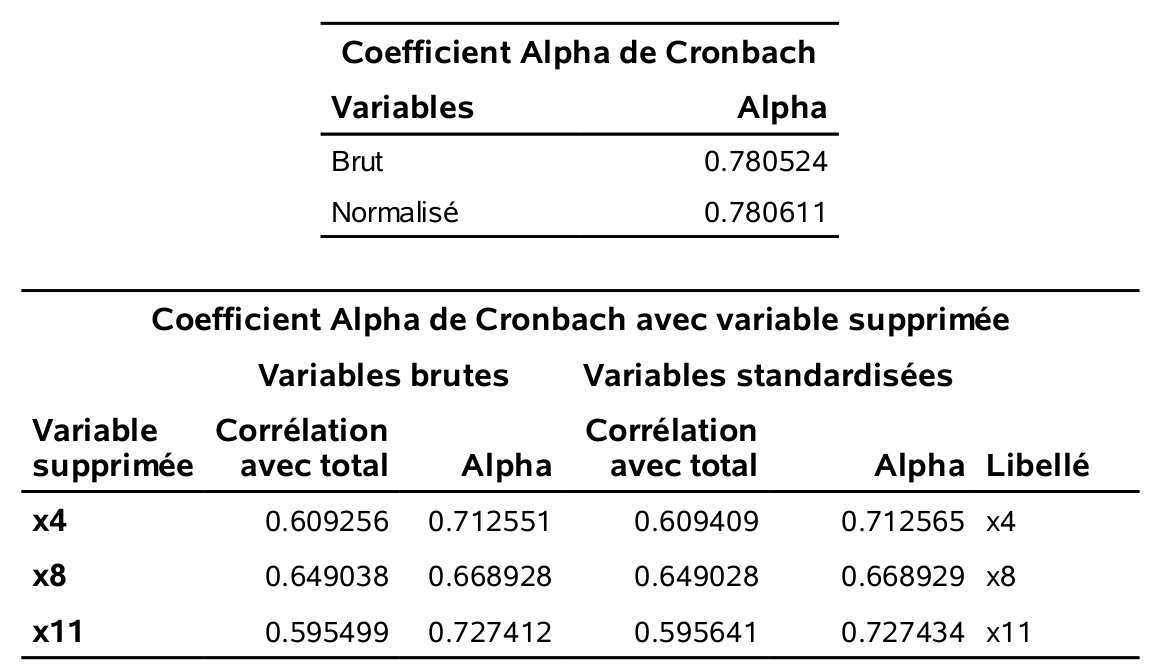
\includegraphics[width=0.85\linewidth]{figures/01-facto-e8} 

}

\caption{Alpha de Cronbach pour le facteur \emph{service}.}\label{fig:fig1p8}
\end{figure}

\begin{figure}

{\centering 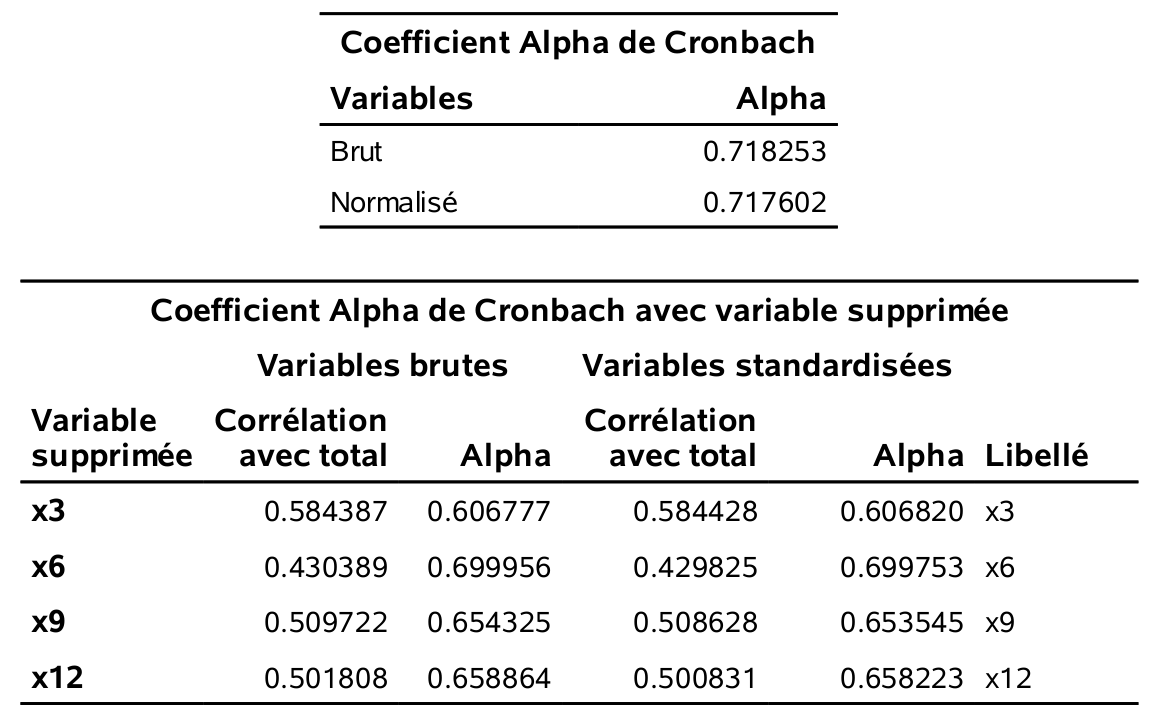
\includegraphics[width=0.85\linewidth]{figures/01-facto-e9} 

}

\caption{Alpha de Cronbach pour le facteur \emph{produits}.}\label{fig:fig1p9}
\end{figure}

\begin{figure}

{\centering 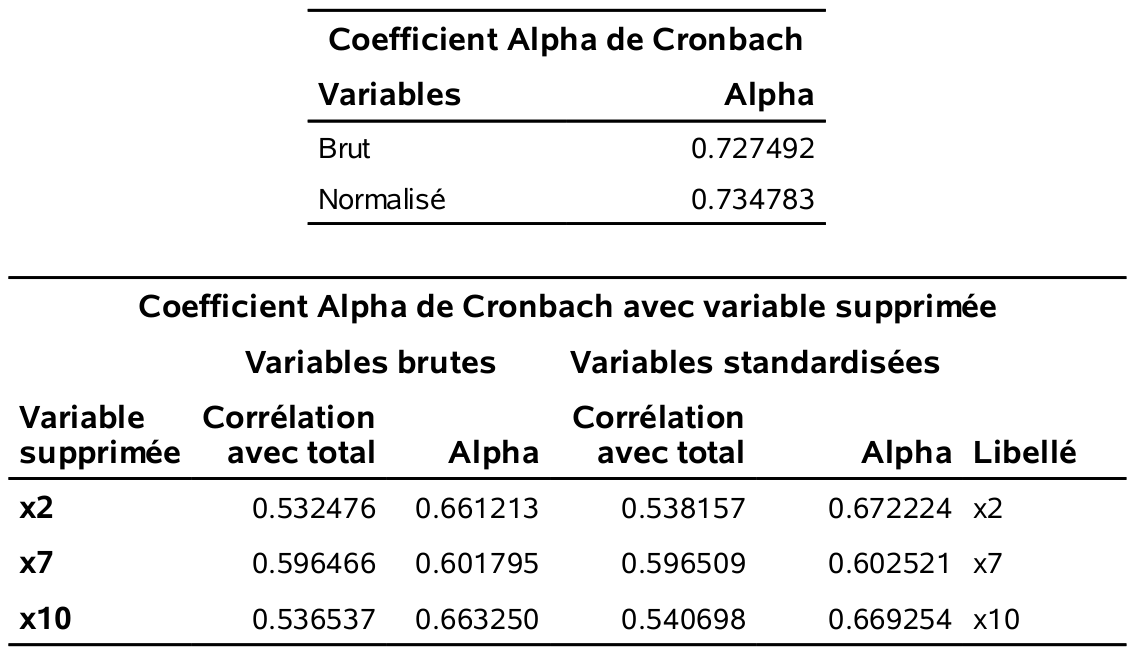
\includegraphics[width=0.85\linewidth]{figures/01-facto-e10} 

}

\caption{Alpha de Cronbach pour le facteur \emph{paiement}.}\label{fig:fig1p10}
\end{figure}

\begin{figure}

{\centering 
\includegraphics[width=0.85\linewidth]{figures/01-facto-e11} 

}

\caption{Alpha de Cronbach pour le facteur \emph{prix}.}\label{fig:fig1p11}
\end{figure}

Il faut utiliser le alpha brut. Ainsi, les alphas de Cronbach sont tous
satisfaisants (plus grand que 0,6) sauf pour le facteur \emph{prix} (\(\alpha=0,546\)). \textsf{SAS}fournit également la matrice des corrélations des variables de l'échelle ainsi que la valeur du alpha de Cronbach si on retirait une variable à la fois de l'échelle. Tout est donc cohérent. Les échelles provenant des facteurs \emph{service}, \emph{produits} et \emph{paiement}, sont satisfaisantes. Ces facteurs sont identifiés à la fois dans la solution à quatre, mais aussi dans la solution à troisfacteurs. Le facteur \emph{prix} est celui qui apparaît en plus dans la solution à quatre facteurs. Il a une interprétation claire, mais son faible alpha ferait en sorte qu'il serait discutable de travailler avec l'échelle \emph{prix} dans d'autres analyses (du moins avec selon l'usage habituel du alpha).

\hypertarget{compluxe9ments-dinformation}{%
\section{Compléments d'information}\label{compluxe9ments-dinformation}}

\hypertarget{variables-ordinales}{%
\subsection{Variables ordinales}\label{variables-ordinales}}

Théoriquement, une analyse factorielle ne devrait être faite qu'avec des
variables continues. Par contre, en pratique, on l'utilise souvent aussi avec des variables ordinales (comme pour l'exemple portant sur le questionnaire) et même avec des variables binaires (0-1).

Dans ce genre de situation, on peut aussi utiliser d'autres mesures d'associations au lieu du coefficient de corrélation linéaire. Par exemple, on peut utiliser la corrélation polychorique, qui est une mesure de corrélation entre deux variables ordinales. La corrélation tétrachorique correspond au cas spécial de deux variables binaires.

Ma suggestion est d'utiliser la corrélation linéaire ordinaire avec des variables ordinales (même binaires). Si les résultats ne sont pas satisfaisants, on peut alors essayer avec d'autres mesures d'associations.

On peut refaire l'analyse des données portant sur le magasin dans \textsf{SAS}en utilisant la corrélation polychorique calculées par la procédure \texttt{corr} et en passant la sortie à la procédure \texttt{factor}.

\begin{verbatim}
proc corr data=multi.factor2 polychoric out=poly_corr;
var x1-x12;
run;

proc factor data=poly_corr
 method=ml rotate=varimax nfact=4
 maxiter=500 flag=.3 hey;
 var x1-x12;
run;
\end{verbatim}

Les chargements sont donnés dans le tableau \ref{fig:fig1p12}. Les facteurs obtenus sont les mêmes qu'en utilisant les corrélations linéaires.

\begin{figure}

{\centering 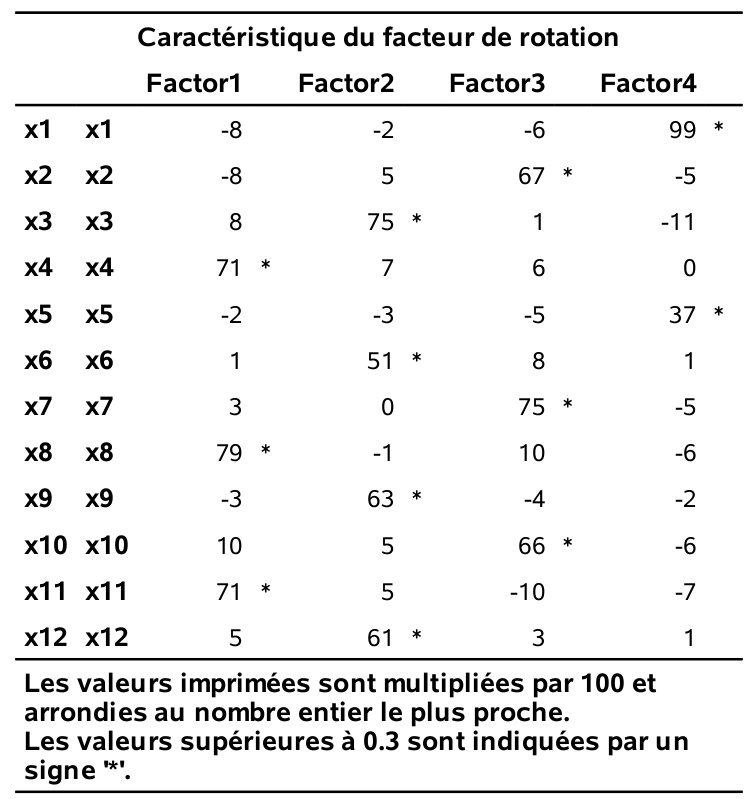
\includegraphics[width=0.65\linewidth]{figures/01-facto-e12} 

}

\caption{Chargements estimés pour la corrélation polychorique}\label{fig:fig1p12}
\end{figure}

\hypertarget{autres-muxe9thodes-dextractions-de-facteurs}{%
\subsection{Autres méthodes d'extractions de facteurs}\label{autres-muxe9thodes-dextractions-de-facteurs}}

Il n'y a pas de formule explicites pour l'estimation des paramètres avec la méthode du maximum de vraisemblance et un algorithme d'optimisation est nécessaire pour l'option des paramètres. Dans certains cas, l'algorithme peut terminer sans solution ou retourner un cas limite (où la variance est négative). La méthode par les composantes principales (mentionnée lors de la présentation des valeurs propres et du diagramme d'éboulis a une solution explicite et peut donc dépanner si on n'arrive pas à obtenir le maximum de vraisemblance.

D'autres méthodes sont aussi disponibles dans \textsf{SAS}(voir la rubrique d'aide du logiciel) mais les deux méthodes mentionnées devraient être suffisantes pour la grande majorité des applications.

\hypertarget{autres-muxe9thodes-de-rotation-des-facteurs}{%
\subsection{Autres méthodes de rotation des facteurs}\label{autres-muxe9thodes-de-rotation-des-facteurs}}

Jusqu'à présent, nous avons utilisé la méthode de rotation orthogonale varimax. Il existe de nombreuses autres méthodes de rotations orthogonales telles, orthomax, quartimax, parsimax et equimax (voir la rubrique d'aide de \textsf{SAS}). Rappelez-vous que le modèle d'analyse factorielle de base suppose que les facteurs sont non corrélés. Les rotations de type obliques quant à elles permettent d'introduire de la corrélation entre les facteurs. Quelquefois, une telle rotation facilitera davantage l'interprétation des facteurs qu'une rotation orthogonale. \textsf{SAS}permet l'utilisation de plusieurs méthodes de
rotation obliques qui sont documentées dans la rubrique d'aide. Notez qu'il faut être prudent lorsqu'on utilise une méthode de rotation oblique car il y aura trois matrices de chargements après rotation. On suggère l'utilisation de la première, soit la représentation avec \textbf{coefficients de régression normalisés}. Il s'agit des coefficients de régression si on voulait prédire les variables à l'aide des facteurs. Ils indiquent donc à quel point chaque facteur est associé à chaque variable. Dans le cas d'une rotation orthogonale, ces trois matrices sont les mêmes et il s'agit de trois interprétations valides des chargements.

Le programme suivant fait une analyse factorielle avec quatre facteurs, mais en utilisant une rotation varimax oblique (option \texttt{rotate=obvarimax}).

\begin{verbatim}
proc factor data=multi.factor2
maxiter=500 flag=.3 hey;
var x1-x12;
run;
\end{verbatim}

La matrice des corrélations entres facteurs est donnée dans le tableau \ref{fig:fig1p13} et les chargements sont présentés dans le tableau \ref{fig:fig1p14}. On voit ici qu'on obtient les mêmes quatre facteurs qu'avec une rotation varimax orthogonale.

\begin{figure}

{\centering 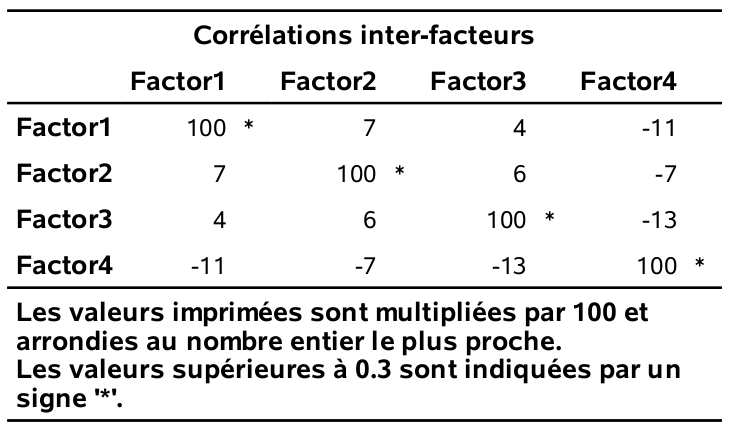
\includegraphics[width=0.7\linewidth]{figures/01-facto-e13} 

}

\caption{Corrélation interfacteurs pour rotation varimax oblique}\label{fig:fig1p13}
\end{figure}

\begin{figure}

{\centering 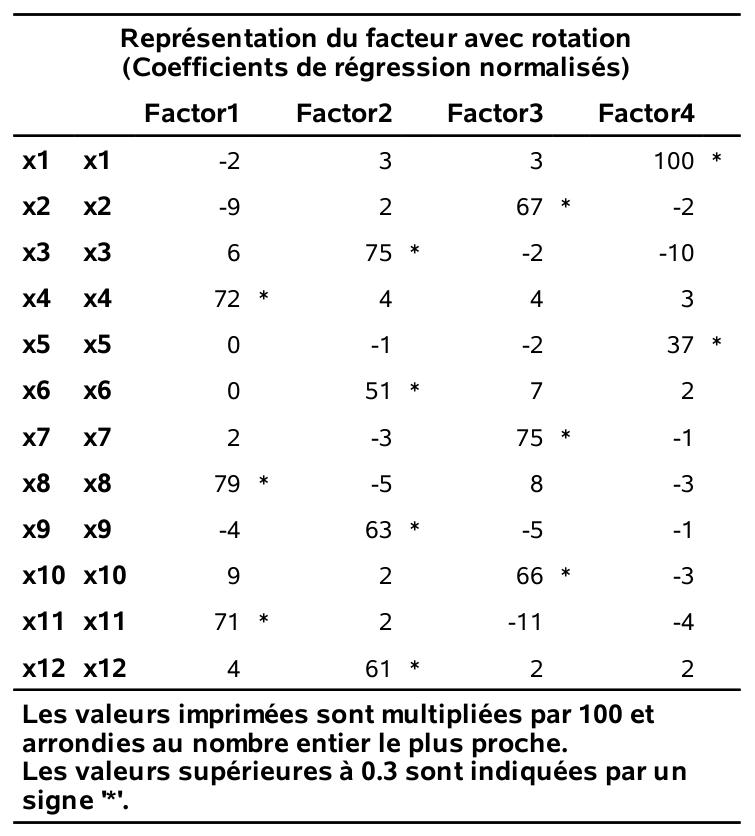
\includegraphics[width=0.7\linewidth]{figures/01-facto-e14} 

}

\caption{Chargements avec rotation oblique varimax}\label{fig:fig1p14}
\end{figure}

\hypertarget{scores-factoriels}{%
\subsection{Scores factoriels}\label{scores-factoriels}}

Avec les données de l'exemple, en nous basant sur les résultats de l'analyse factorielle, nous avons créé quatre nouvelles échelles (une par facteur) que l'on peut calculer pour chaque individu:

\begin{itemize}
\tightlist
\item
  \emph{service} = \((X_4+X_8+X_{11})/3\),
\item
  \emph{produit} = \((X_3+X_6+X_9+X_{12})/4\),
\item
  \emph{paiement} = \((X_2+X_7+X_{10})/3\),
\item
  \emph{prix} = \((X_1+X_5)/2\).
\end{itemize}

Par exemple, la variable \emph{prix} peut donc être vu comme une combinaison linéaire des 12
variables où seulement \(X_1\) et \(X_5\) reçoivent un poids (égal) différent de zéro. Une autre façon de créer de nouvelles variables consiste à calculer des scores factoriels (un pour chaque facteur) pour chaque individu. Par exemple, pour un individu donné, un score factoriel pour le premier facteur peut être calculé selon la formule
\begin{align*}
\hat{F}_1 = \widehat{\beta}_1 x_1 + \cdots + \widehat{\beta}_{12}x_{12},
\end{align*}
où \(x_1, \ldots, x_{12}\) sont les valeurs (habituellement standardisées) des variables pour cet individu et où \(\widehat{\beta}_1, \ldots, \widehat{\beta}_{12}\) sont des coefficients estimés à partir des chargements (après rotation) et de la matrice de corrélation des variables.

Ainsi, chacune des 12 variables originales contribue au calcul du score
factoriel. Les variables ayant des chargements plus élevés sur ce facteur auront tendance à avoir des poids (\(\widehat{\beta}\)) plus élevés. Par contre, les scores factoriels ne sont pas uniques car ils dépendent des chargements utilisés (et donc à la fois de la méthode d'estimation et de la méthode de rotation).
On peut également utiliser les scores factoriels au lieu des 12 variables
originales dans des analyses subséquentes. Il est suggéré d'utiliser les nouvelles variables (échelles) obtenues en faisant les moyennes des variables identifiées comme faisant partie de chaque
facteur pour les raisons suivantes:

\begin{itemize}
\tightlist
\item
  l'interprétation des scores factoriels est moins claire (chaque facteur dépend de toutes les variables)
\item
  les scores factoriels ne sont pas uniques (ils dépendent de la méthode d'estimation et de rotation).
\item
  les coefficients servant au calcul seront différents d'une étude à l'autre.
\end{itemize}

\begin{figure}

{\centering 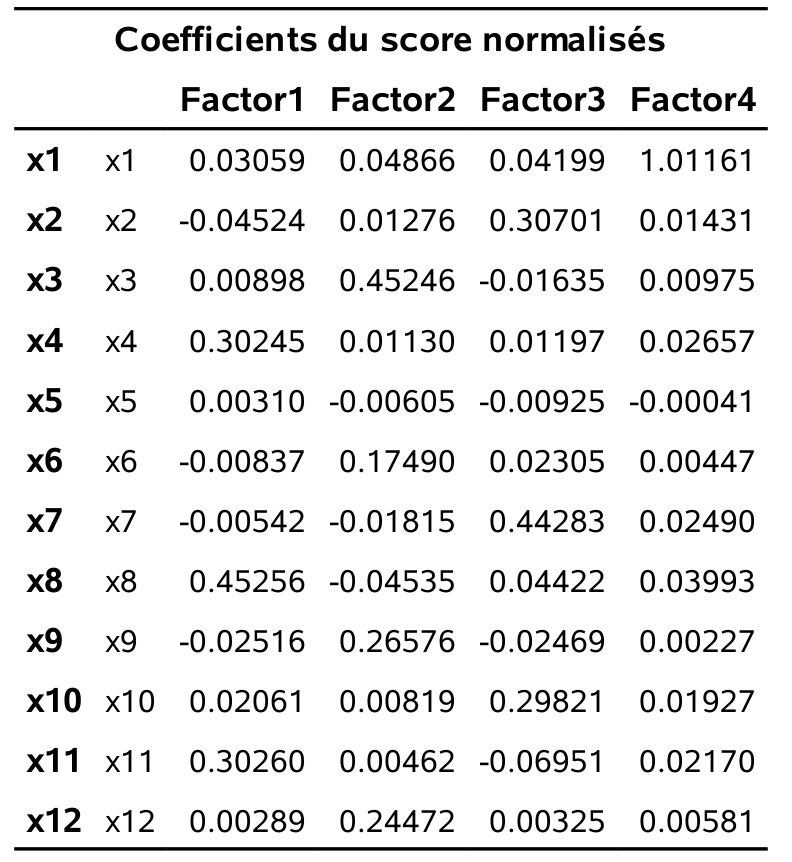
\includegraphics[width=0.6\linewidth]{figures/01-facto-e15} 

}

\caption{Coefficients du score normalisés}\label{fig:fig1p15}
\end{figure}

Pour obtenir les scores avec \textsf{SAS}, il suffit d'insérer l'option \texttt{score} à la procédure \texttt{factor}. L'option \texttt{out=...} permet de créer un fichier de données \textsf{SAS}qui contient la valeur des \(m\) scores pour chaque individu.
Les scores factoriels pour l'exemples sont rapportés dans le tableau \ref{fig:fig1p15}. On remarque que

\begin{itemize}
\tightlist
\item
  pour le premier facteur, trois variables ont des poids importants (\(X_4\), \(X_8\) et \(X_{11}\)). Il s'agit donc d'un facteur très proche du facteur \emph{service}.
\item
  pour le deuxième facteur, les variables \(X_3\), \(X_6\), \(X_9\) et \(X_{12}\) ont des poids importants. Il s'agit donc d'un facteur très proche du facteur \emph{produits}.
\item
  pour le troisième facteur, les variables \(X_2\), \(X_7\), \(X_{10}\) ont des poids importants. Il s'agit donc d'un facteur très proche du facteur \emph{paiement}.
\item
  pour le quatrième facteur, seule la variable \(X_1\) a un poids important.
  On aurait pu s'attendre à ce que ce soit également le cas pour \(X_5\), en lien avec le facteur \emph{prix} --- ce facteur était moins clair selon le alpha de Cronbach.
\end{itemize}

Les corrélations entre les échelles (construites avec les moyennes) et les scores factoriels sont données dans le tableau \ref{fig:fig1p16}. On remarque la forte corrélation entre le score factoriel et les échelles construites avec les moyennes pour les facteurs \emph{service}, \emph{produits} et
\emph{paiement}. Cela veut dire qu'utiliser les échelles ou les scores factoriels ne
devrait pas faire de différence dans des analyses subséquentes. Par contre,
cette corrélation est plus faible (0.82) pour le facteur \emph{prix}.

\begin{figure}

{\centering 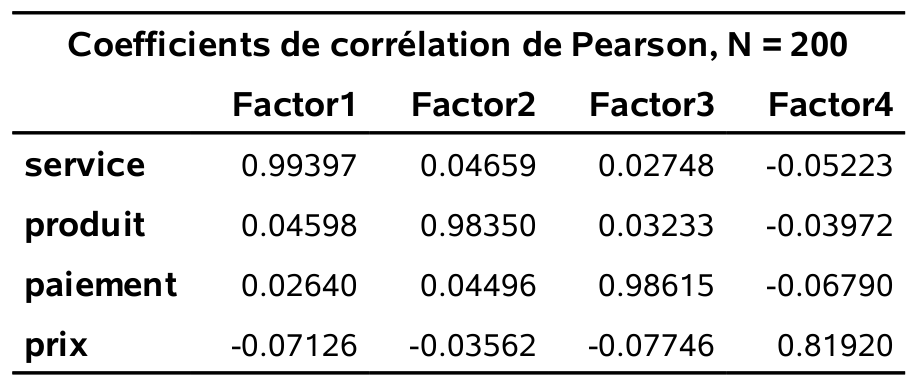
\includegraphics[width=0.65\linewidth]{figures/01-facto-e16} 

}

\caption{Corrélation entre scores et échelles}\label{fig:fig1p16}
\end{figure}

\backmatter
  \bibliography{book.bib,packages.bib}

\end{document}
